\subsection{CU1 Iniciar Sesión}
Esta pantalla (figura \ref{fig:Pantalla Iniciar Sesion - Vista de Escenarios}) será la primera en aparecer al ejecutarse el sistema. Se compone de un pequeño formulario donde el usuario (Mecánico) deberá teclear sus credenciales otorgadas por la administración de la empresa. Una vez ingresados de manera correcta, deberá pulsar el botón 'Ingresar'.
\\
En caso de que el usuario desee salir del sistema, solo deberá pulsar el botón 'Salir'. 
\\

\begin{figure}[!h]
	\centering
	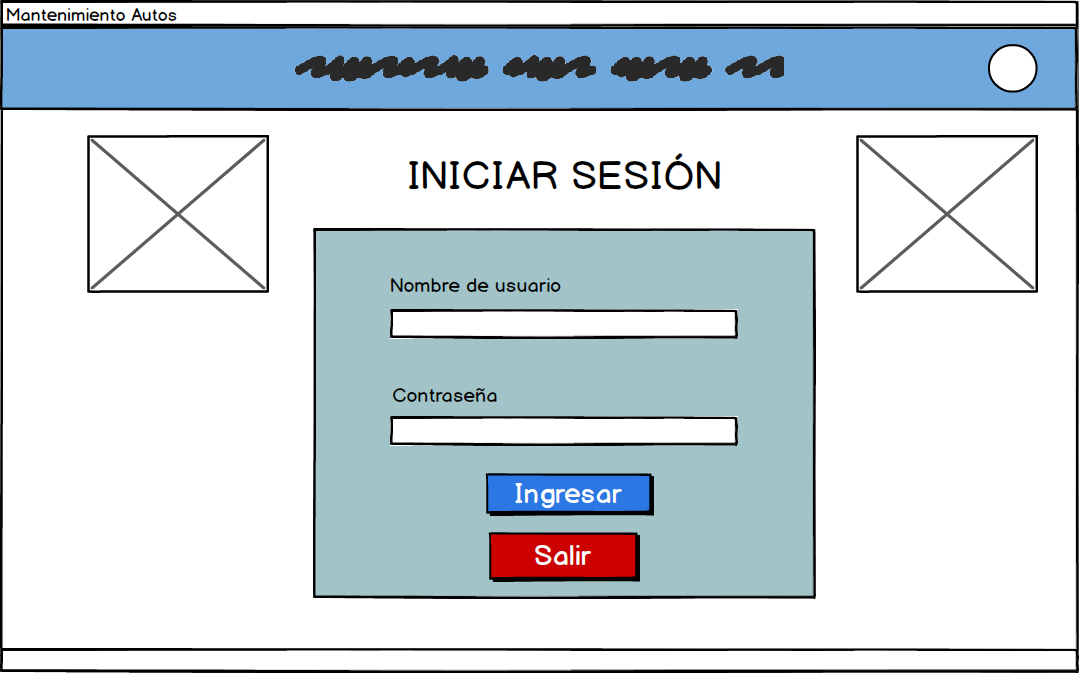
\includegraphics[width=1\textwidth]{./diseno/vescenarios/imagenes/Login}
	\caption{Pantalla Iniciar Sesión - Vista de Escenarios}
	\label{fig:Pantalla Iniciar Sesion - Vista de Escenarios}
\end{figure}
En ese sentido, si el usuario ingresa erróneamente sus credenciales de autenticación, el sistema mostrará un mensaje de alerta (\ref{fig:Alerta1 - Vista de Escenarios}).
\\
\begin{figure}[!h]
	\centering
	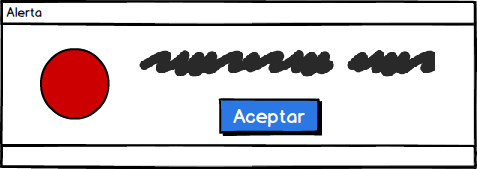
\includegraphics[width=0.5\textwidth]{./diseno/vescenarios/imagenes/alerta}
	\caption{Alerta Datos Erróneos - Vista de Escenarios}
	\label{fig:Alerta1 - Vista de Escenarios}
\end{figure}
\clearpage